\documentclass[a4paper, oneside,11pt]{article}
\usepackage[a4paper,top=3cm,bottom=3cm,left=3cm,right=3cm,marginparwidth=1.75cm]{geometry}
\usepackage[utf8]{inputenc}
\usepackage{lipsum}
\usepackage{graphicx}
\usepackage{times}
\usepackage{xcolor}
%\usepackage{booktabs}
\usepackage{float}
\usepackage{color}
\usepackage{hyperref}
\usepackage{amsmath}
%\usepackage{subfig}
\usepackage{subcaption}
\usepackage[backend=biber,
    style=numeric,sorting=none]{biblatex}
\addbibresource{ref.bib}
\hypersetup{
    colorlinks=true,
    linkcolor=blue,
    urlcolor=blue,
}
\graphicspath{{/}}
\usepackage{adjustbox}
\usepackage{tabularx}
\usepackage{multirow}
\usepackage{titlesec}
\usepackage{graphicx}
\usepackage{upgreek}
\usepackage{enumitem}  
\usepackage{comment} 
\usepackage{upgreek}

%%%%%%%%%%%%%%%%%%%%%%%%%%%%%%%%%%%%%%%%%%%%%%%%%%%%%%%%%%%%%%%%%%%%

\begin{document}

\begin{table}[h]
		\begin{adjustbox}{width = \linewidth}
			\begin{tabular}{c c c}
				\multirow{5}{*}{ 
\includegraphics[width=0.13\textwidth]{iitb_logo.png}} \hfill &  \large{{Institute Technical Summer Project}}  & \hfill \multirow{5}{*}{ 
\includegraphics[width=0.13\textwidth]{itc_logo.png}} \\
				& {Indian Institute of Technology, Bombay} &\\
				& {Powai, Mumbai - 400076, INDIA} &\\
				&{} &\\
				& Website: {https://github.com/bvcxz1/ITSP} &\\
				\\
				&\large{\textbf{Formulae - itsp.py}}&\\
				&Writing in Thin Air&\\
				\hline
			\end{tabular}
		\end{adjustbox}
\end{table}

\textbf{Signal Processing:}

\begin{itemize}

	\item \textbf{Transformation Matrix}
		A transformation matrix is used to reduce the number of dimensions of the acceleration input from 3 to 2 by eliminating the null space in the signal input.

		The first matrix changes the frame of reference from the body frame of the sensor to an inertial frame
		\begin{eqnarray}
		T_1 & \rightarrow
		  \begin{bmatrix}
			x_1\\
			y_1\\
			z_0
		  \end{bmatrix}
		  =
		  \left[
		  \begin{matrix}
			cos \theta & -sin \theta & 0\\
			sin \theta & cos \theta & 0\\
			0 & 0 & 1
		  \end{matrix}
		  \right]
		  \left[
		  \begin{matrix}
			x_0\\
			y_0\\
			z_0
		  \end{matrix}
		  \right]
		\end{eqnarray}

		The second matrix eliminates the null space
		\begin{eqnarray}
		T_2 & \rightarrow
		  \begin{bmatrix}
			x_2\\
			y_1\\
			0
		  \end{bmatrix}
		  =
		  \left[
		  \begin{matrix}
			cos \phi & 0 & sin \phi \\
			0 & 1 & 0\\
			-sin \phi & 0 & cos \phi
		  \end{matrix}
		  \right]
		  \left[
		  \begin{matrix}
			x_1\\
			y_1\\
			z_0
		  \end{matrix}
		  \right]
		\end{eqnarray}
		where \begin{math}\left[x_2\ y_1\ 0\right]^t\end{math} is called \textit{sensor\_output\_red}

	\item \textbf{Moving Average Filter:}
		A filter used to remove high frequency noise from raw data
		\begin{eqnarray}
		   filtered\_output\_ma_i = \frac{1}{n} \sum_{j=i}^{i+n} sensor\_output\_red_j \ \forall \ i \ \in \left[ \  0,\ N - n \ \right]
		\end{eqnarray}
		where n is a variable over which the number of recent readings are averaged

	\item \textbf{High Pass Filter:}
		A filter used to remove gravitational acceleration from raw data 
		\begin{eqnarray}
		  filtered\_output\_hp = filtered\_output\_ma - \textit{g}
		\end{eqnarray}
		where \textit{g} is the acceleration due to gravity
\end{itemize}

\textbf{Image Generation:}

\begin{itemize}
	\item \textbf{Velocity}
		\begin{eqnarray}
		  v_i = v_{i-1} + \frac{(a_i + a_{i-1})}{2}*t
		\end{eqnarray}
		acceleration is assumed to be \textit{piece-wise} linear and the area under the line is found

	\item \textbf{Position}
		\begin{eqnarray}
		  r_i = r_{i-1} + \frac{(v_i + v_{i-1})}{2}*t
		\end{eqnarray}
\end{itemize}

\textbf{Neural Network:}

\begin{itemize}
	\item \textbf{Sigmoid Neurons, \textit{also called logistic neurons}}

		The sigmoid neuron has inputs, \begin{math}x_1, x_2, \ldots \end{math}which can take on any values between 0 and 1. So, for instance, \begin{math}0.4238\ldots \end{math}is a valid input for a sigmoid neuron. The sigmoid neuron has weights for each input, \begin{math}w_1, w_2, \ldots, \end{math}and an overall bias, b.  The output of \begin{math}\sigma(w \cdot x+b)\end{math} will be between 0 and 1, and is called the \textit{sigmoid or logistic function}.
		\begin{eqnarray} 
		  \sigma(z) \equiv \frac{1}{1+e^{-z}}.
		\end{eqnarray}
		\begin{eqnarray} 
		  \sigma(z) \equiv \frac{1}{1+\exp(-\sum_j w_j x_j-b)}.
		\end{eqnarray}
		The shape of the sigmoid function when plotted:
		\begin{center}
			\large{ 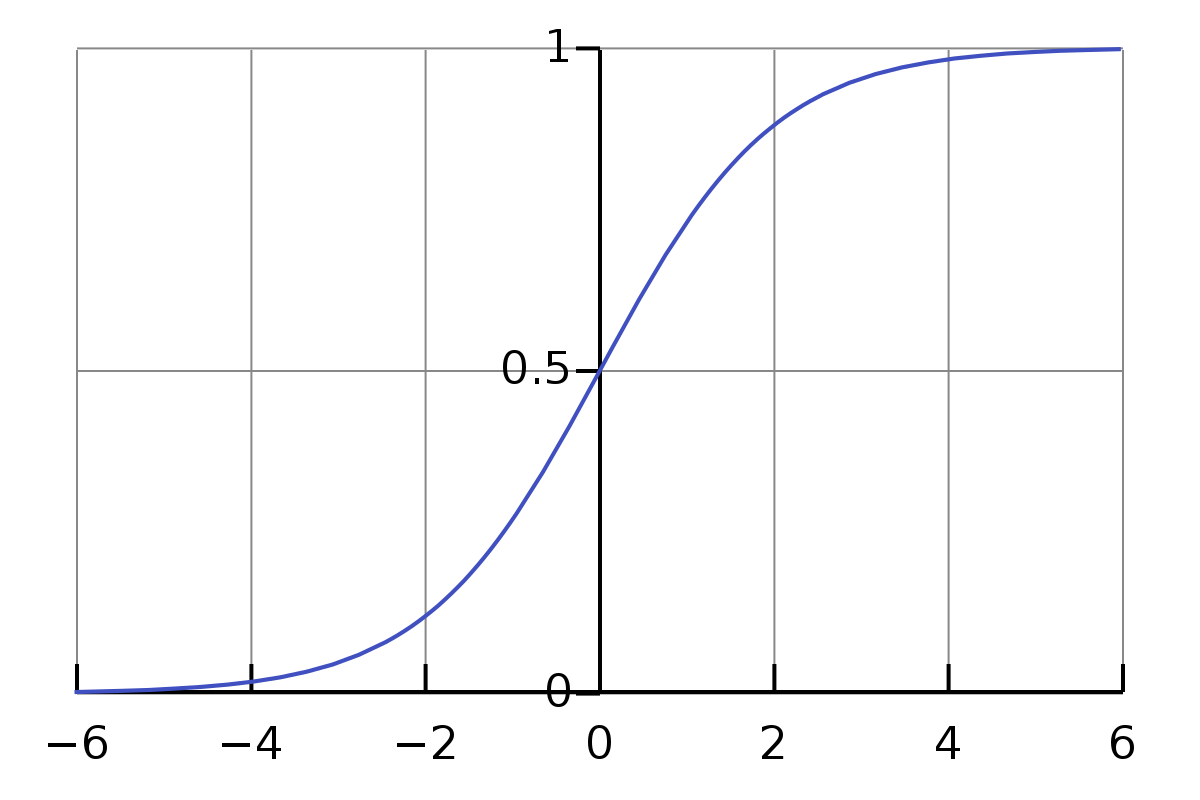
\includegraphics[width=0.5\textwidth]{sigmoid_function.png}}
		\end{center}
		The smoothness of \begin{math}\sigma\end{math} means that small changes \begin{math}\Delta w_j\end{math} in the weights and \begin{math}\Delta b\end{math} in the bias will produce a small change \begin{math}\Delta output\end{math} in the output from the neuron. In fact, calculus tells us that \begin{math}\Delta output\end{math} is well approximated by:
		\begin{eqnarray} 
		  \Delta \mbox{output} \approx \sum_j \frac{\partial \, \mbox{output}}{\partial w_j}
  		  \Delta w_j + \frac{\partial \, \mbox{output}}{\partial b} \Delta b,
		\end{eqnarray}
		where the sum is over all the weights, \begin{math}w_j\end{math}, and \begin{math}\delta output/\delta w_j\end{math} and \begin{math}\delta output/\delta b\end{math} denote partial derivatives of the output with respect to \begin{math}w_j\end{math} and b, respectively.

	\item \textbf{Cost Function, \textit{also called loss or objective function}}
		To find weights and biases so that the output from the network approximates \begin{math}y(x)\end{math} for all training inputs \begin{math}x\end{math}:
		\begin{eqnarray}  C(w,b) \equiv
		  \frac{1}{2n} \sum_x \| y(x) - a\|^2.
		\end{eqnarray}
		Here, \begin{math}n\end{math}  is the total number of training inputs, \begin{math}a\end{math} is the vector of outputs from the network when \begin{math}x\end{math} is input, and the sum is over all training inputs, \begin{math}x\end{math} and \begin{math}C\end{math}  is called the quadratic cost function; it's also sometimes known as the \textit{mean squared error} or just \textit{MSE}.
		The aim of a training algorithm will be to minimize the cost function and will be done using an algorithm known as gradient descent.		

	\item \textbf{Learning Rate}
		For small changes
		\begin{eqnarray} 
		  \Delta C \approx \nabla C \cdot \Delta v.
		\end{eqnarray}
		If we choose
		\begin{eqnarray} 
		  \Delta v = -\eta \nabla C,
		  v \rightarrow v' = v-\eta \nabla C.
		\end{eqnarray}
		where \begin{math}\eta\end{math} is a small, positive parameter known as the learning rate then
		\begin{eqnarray}
		  \Delta C \approx -\eta
		  \nabla C \cdot \nabla C = -\eta \|\nabla C\|^2
		\end{eqnarray}
		and this guarantees that \begin{math}\Delta C \leq 0\end{math}, i.e., \begin{math}C\end{math} will always decrease. To make gradient descent work correctly, \begin{math}\eta\end{math}is chosen to be small enough that Equation 11) is a good approximation and \begin{math}\Delta C \leq 0\end{math} holds true. At the same time, \begin{math}\eta\end{math} can't be too small and the gradient descent algorithm will work very slowly.

	\item \textbf{Applying Gradient Descent}
		The idea is to use gradient descent to find the weights \begin{math}w_k\end{math} and biases \begin{math}b_l\end{math} which minimize the cost in Equation (10). Writing out the gradient descent update rule in terms of components:
		\begin{eqnarray}
		  w_k & \rightarrow & w_k' = w_k-\eta \frac{\partial C}{\partial w_k} \\
		  b_l & \rightarrow & b_l' = b_l-\eta \frac{\partial C}{\partial b_l}.
		\end{eqnarray}
		The code implements a minimised version of Gradient Descent called the Stochastic Gradient Descent where the average value is not calculated for all the values but only for a few randomly chosen values.
	\item \textbf{Mini Batch Size}
		The factor by which the number of elements is reduced to apply Stochastic Gradient Descent
	\item \textbf{Epoch}
		The point at which all training inputs have been exhausted
\end{itemize}

\printbibliography 
\end{document}
